% !TEX root = ./main.tex
% ^ Tells LaTeX Workshop (Cursor/VSCode) to treat this file as the build root.
% Needed because \documentclass lives in arena_beamer.sty (\input'ed below)
% rather than in this file, and the extension's root-file detector greps for
% \documentclass without following \input -- so without this line it reports
% "No root file found" and silently aborts Ctrl+Alt+B. CLI builds are
% unaffected; latexmk/pdflatex follow \input fine.
% Local-dev build-mode toggle. 1 = handout (all \pause overlays collapsed,
% small PDF), 0 = presentation (each \pause becomes an extra page, for
% live talks). CI overrides this via latexmk -usepretex regardless of what
% it's set to here, so this line only affects local pdflatex/latexmk runs.
\providecommand{\HANDOUT}{1}
% arena_beamer.sty - shared preamble for all ARENA talk decks.
%
% Loaded BEFORE \documentclass (via plain \input, not \usepackage) so that
% it can decide whether to pass `handout` to beamer based on the \HANDOUT
% toggle. The deck pattern is:
%
%   \providecommand{\HANDOUT}{1}              % 1 = handout, 0 = presentation
%   % arena_beamer.sty - shared preamble for all ARENA talk decks.
%
% Loaded BEFORE \documentclass (via plain \input, not \usepackage) so that
% it can decide whether to pass `handout` to beamer based on the \HANDOUT
% toggle. The deck pattern is:
%
%   \providecommand{\HANDOUT}{1}              % 1 = handout, 0 = presentation
%   % arena_beamer.sty - shared preamble for all ARENA talk decks.
%
% Loaded BEFORE \documentclass (via plain \input, not \usepackage) so that
% it can decide whether to pass `handout` to beamer based on the \HANDOUT
% toggle. The deck pattern is:
%
%   \providecommand{\HANDOUT}{1}              % 1 = handout, 0 = presentation
%   \input{../../arena_beamer.sty}
%   ... deck-local macros ...
%   \begin{document} ... \end{document}
%
% CI overrides the deck's local toggle via latexmk's -usepretex flag, which
% \def's \HANDOUT before main.tex starts. The \providecommand below is a
% safety default if neither the deck nor CI set anything.

\providecommand{\HANDOUT}{1}
\ifnum\HANDOUT=1
  \PassOptionsToClass{handout}{beamer}
\fi
\documentclass[10pt,a4paper]{beamer}

\RequirePackage[latin1]{inputenc}
\RequirePackage{amsmath}
\RequirePackage{amsfonts}
\RequirePackage{amssymb}
\RequirePackage{graphicx}
\RequirePackage{ulem}
\RequirePackage{algorithm2e}
\RequirePackage{algpseudocode}
\RequirePackage{diffcoeff}
\RequirePackage{xcolor}
\RequirePackage{tikz}
\RequirePackage{cancel}
\RequirePackage{pgfplots}
\RequirePackage{background}
\RequirePackage{stmaryrd}
\RequirePackage{subcaption}
\RequirePackage{ifthen}
\RequirePackage{listings}
\RequirePackage{hyperref}

\usetheme{Madrid}

\hypersetup{
    colorlinks=true,
    linkcolor=white,
    filecolor=magenta,
    urlcolor=cyan,
}
\urlstyle{same}

\DeclareMathOperator*{\argmin}{\arg\!\min}
\DeclareMathOperator*{\argmax}{arg\,max}

\usetikzlibrary{calc, fadings, decorations.pathreplacing, automata, positioning, arrows, shapes.geometric, arrows.meta, positioning, fit, backgrounds}

% Generic math/style macros used across decks.
% Anything chapter-specific (state space, reward set, etc.) lives in the
% deck's own main.tex, not here.
\newcommand{\Ex}{\mathbb{E}}
\newcommand{\red}[1]{\textcolor{red}{#1}}
\newcommand{\bth}{{\boldsymbol{\theta}}}

% PyTorch code listing style.
\definecolor{codegreen}{rgb}{0,0.5,0}
\definecolor{codegray}{rgb}{0.4,0.4,0.4}
\definecolor{codepurple}{rgb}{0.55,0.0,0.55}
\definecolor{codeblue}{rgb}{0.0,0.0,0.6}

\lstdefinestyle{pystyle}{
    basicstyle=\ttfamily\scriptsize,
    keywordstyle=\color{codeblue}\bfseries,
    commentstyle=\color{codegreen}\itshape,
    stringstyle=\color{codepurple},
    numberstyle=\tiny\color{codegray},
    breaklines=true,
    showstringspaces=false,
    language=Python,
    morekeywords={self, nn, torch, Tensor},
    columns=fullflexible,
    keepspaces=true,
}
\lstset{style=pystyle}

% Decks set their own \graphicspath after \usepackage{arena_beamer}, but
% default to img/ so plain \includegraphics works without ceremony.
\graphicspath{{img/}}

% Falls back to a labeled placeholder box if the image file isn't present.
% Usage: \imgorplaceholder{0.6\linewidth}{filename-no-ext}{Caption shown if missing}
\newcommand{\imgorplaceholder}[3]{%
    \IfFileExists{img/#2.png}{\includegraphics[width=#1]{#2}}{%
    \IfFileExists{img/#2.jpg}{\includegraphics[width=#1]{#2}}{%
    \IfFileExists{img/#2.pdf}{\includegraphics[width=#1]{#2}}{%
    \IfFileExists{img/#2.svg}{\includegraphics[width=#1]{#2}}{%
        \fbox{\parbox[c][0.45\textheight][c]{#1}{\centering \textit{[image: #3]}\\\scriptsize drop \texttt{img/#2.(png|jpg|pdf)}}}%
    }}}}%
}

\endinput

%   ... deck-local macros ...
%   \begin{document} ... \end{document}
%
% CI overrides the deck's local toggle via latexmk's -usepretex flag, which
% \def's \HANDOUT before main.tex starts. The \providecommand below is a
% safety default if neither the deck nor CI set anything.

\providecommand{\HANDOUT}{1}
\ifnum\HANDOUT=1
  \PassOptionsToClass{handout}{beamer}
\fi
\documentclass[10pt,a4paper]{beamer}

\RequirePackage[latin1]{inputenc}
\RequirePackage{amsmath}
\RequirePackage{amsfonts}
\RequirePackage{amssymb}
\RequirePackage{graphicx}
\RequirePackage{ulem}
\RequirePackage{algorithm2e}
\RequirePackage{algpseudocode}
\RequirePackage{diffcoeff}
\RequirePackage{xcolor}
\RequirePackage{tikz}
\RequirePackage{cancel}
\RequirePackage{pgfplots}
\RequirePackage{background}
\RequirePackage{stmaryrd}
\RequirePackage{subcaption}
\RequirePackage{ifthen}
\RequirePackage{listings}
\RequirePackage{hyperref}

\usetheme{Madrid}

\hypersetup{
    colorlinks=true,
    linkcolor=white,
    filecolor=magenta,
    urlcolor=cyan,
}
\urlstyle{same}

\DeclareMathOperator*{\argmin}{\arg\!\min}
\DeclareMathOperator*{\argmax}{arg\,max}

\usetikzlibrary{calc, fadings, decorations.pathreplacing, automata, positioning, arrows, shapes.geometric, arrows.meta, positioning, fit, backgrounds}

% Generic math/style macros used across decks.
% Anything chapter-specific (state space, reward set, etc.) lives in the
% deck's own main.tex, not here.
\newcommand{\Ex}{\mathbb{E}}
\newcommand{\red}[1]{\textcolor{red}{#1}}
\newcommand{\bth}{{\boldsymbol{\theta}}}

% PyTorch code listing style.
\definecolor{codegreen}{rgb}{0,0.5,0}
\definecolor{codegray}{rgb}{0.4,0.4,0.4}
\definecolor{codepurple}{rgb}{0.55,0.0,0.55}
\definecolor{codeblue}{rgb}{0.0,0.0,0.6}

\lstdefinestyle{pystyle}{
    basicstyle=\ttfamily\scriptsize,
    keywordstyle=\color{codeblue}\bfseries,
    commentstyle=\color{codegreen}\itshape,
    stringstyle=\color{codepurple},
    numberstyle=\tiny\color{codegray},
    breaklines=true,
    showstringspaces=false,
    language=Python,
    morekeywords={self, nn, torch, Tensor},
    columns=fullflexible,
    keepspaces=true,
}
\lstset{style=pystyle}

% Decks set their own \graphicspath after \usepackage{arena_beamer}, but
% default to img/ so plain \includegraphics works without ceremony.
\graphicspath{{img/}}

% Falls back to a labeled placeholder box if the image file isn't present.
% Usage: \imgorplaceholder{0.6\linewidth}{filename-no-ext}{Caption shown if missing}
\newcommand{\imgorplaceholder}[3]{%
    \IfFileExists{img/#2.png}{\includegraphics[width=#1]{#2}}{%
    \IfFileExists{img/#2.jpg}{\includegraphics[width=#1]{#2}}{%
    \IfFileExists{img/#2.pdf}{\includegraphics[width=#1]{#2}}{%
    \IfFileExists{img/#2.svg}{\includegraphics[width=#1]{#2}}{%
        \fbox{\parbox[c][0.45\textheight][c]{#1}{\centering \textit{[image: #3]}\\\scriptsize drop \texttt{img/#2.(png|jpg|pdf)}}}%
    }}}}%
}

\endinput

%   ... deck-local macros ...
%   \begin{document} ... \end{document}
%
% CI overrides the deck's local toggle via latexmk's -usepretex flag, which
% \def's \HANDOUT before main.tex starts. The \providecommand below is a
% safety default if neither the deck nor CI set anything.

\providecommand{\HANDOUT}{1}
\ifnum\HANDOUT=1
  \PassOptionsToClass{handout}{beamer}
\fi
\documentclass[10pt,a4paper]{beamer}

\RequirePackage[latin1]{inputenc}
\RequirePackage{amsmath}
\RequirePackage{amsfonts}
\RequirePackage{amssymb}
\RequirePackage{graphicx}
\RequirePackage{ulem}
\RequirePackage{algorithm2e}
\RequirePackage{algpseudocode}
\RequirePackage{diffcoeff}
\RequirePackage{xcolor}
\RequirePackage{tikz}
\RequirePackage{cancel}
\RequirePackage{pgfplots}
\RequirePackage{background}
\RequirePackage{stmaryrd}
\RequirePackage{subcaption}
\RequirePackage{ifthen}
\RequirePackage{listings}
\RequirePackage{hyperref}

\usetheme{Madrid}

\hypersetup{
    colorlinks=true,
    linkcolor=white,
    filecolor=magenta,
    urlcolor=cyan,
}
\urlstyle{same}

\DeclareMathOperator*{\argmin}{\arg\!\min}
\DeclareMathOperator*{\argmax}{arg\,max}

\usetikzlibrary{calc, fadings, decorations.pathreplacing, automata, positioning, arrows, shapes.geometric, arrows.meta, positioning, fit, backgrounds}

% Generic math/style macros used across decks.
% Anything chapter-specific (state space, reward set, etc.) lives in the
% deck's own main.tex, not here.
\newcommand{\Ex}{\mathbb{E}}
\newcommand{\red}[1]{\textcolor{red}{#1}}
\newcommand{\bth}{{\boldsymbol{\theta}}}

% PyTorch code listing style.
\definecolor{codegreen}{rgb}{0,0.5,0}
\definecolor{codegray}{rgb}{0.4,0.4,0.4}
\definecolor{codepurple}{rgb}{0.55,0.0,0.55}
\definecolor{codeblue}{rgb}{0.0,0.0,0.6}

\lstdefinestyle{pystyle}{
    basicstyle=\ttfamily\scriptsize,
    keywordstyle=\color{codeblue}\bfseries,
    commentstyle=\color{codegreen}\itshape,
    stringstyle=\color{codepurple},
    numberstyle=\tiny\color{codegray},
    breaklines=true,
    showstringspaces=false,
    language=Python,
    morekeywords={self, nn, torch, Tensor},
    columns=fullflexible,
    keepspaces=true,
}
\lstset{style=pystyle}

% Decks set their own \graphicspath after \usepackage{arena_beamer}, but
% default to img/ so plain \includegraphics works without ceremony.
\graphicspath{{img/}}

% Falls back to a labeled placeholder box if the image file isn't present.
% Usage: \imgorplaceholder{0.6\linewidth}{filename-no-ext}{Caption shown if missing}
\newcommand{\imgorplaceholder}[3]{%
    \IfFileExists{img/#2.png}{\includegraphics[width=#1]{#2}}{%
    \IfFileExists{img/#2.jpg}{\includegraphics[width=#1]{#2}}{%
    \IfFileExists{img/#2.pdf}{\includegraphics[width=#1]{#2}}{%
    \IfFileExists{img/#2.svg}{\includegraphics[width=#1]{#2}}{%
        \fbox{\parbox[c][0.45\textheight][c]{#1}{\centering \textit{[image: #3]}\\\scriptsize drop \texttt{img/#2.(png|jpg|pdf)}}}%
    }}}}%
}

\endinput


% Deck-local macros (RL chapter math notation).
\newcommand{\R}{\mathcal{R}}
\renewcommand{\S}{\mathcal{S}}
\newcommand{\A}{\mathcal{A}}
\renewcommand{\Pr}{\text{Pr}}
\renewcommand{\P}{\text{P}}
\newcommand{\iter}{\xrightarrow{I}}
\newcommand{\eval}{\xrightarrow{E}}
\newcommand{\iver}[1]{\llbracket {#1} \rrbracket}
\newcommand{\biject}{\langle \cdot \rangle}
\newcommand{\bij}[1]{\langle {#1} \rangle}
\newcommand{\pth}{{\boldsymbol{\phi}}}
\newcommand{\eps}{\epsilon}
\newcommand{\eplen}{T}
\newcommand{\env}{\mu}
\algnewcommand\algorithmicinput{\textbf{Input:}}
\algnewcommand\Input{\item[\algorithmicinput]}
\algnewcommand\algorithmicoutput{\textbf{Output:}}
\algnewcommand\Output{\item[\algorithmicoutput]}
\algnewcommand\algorithmiceffect{\textbf{Effect:}}
\algnewcommand\Effect{\item[\algorithmiceffect]}

\begin{document}

\title[{[2.3] PPO}]
{{[2.3] PPO}}

 
\author[David Quarel] % (optional, for multiple authors)
{David Quarel}
 
\institute[ARENA-5] % (optional)
{
  oh no lots of maths in this one :(
}
 
% \date[23rd Jan 2024] % (optional)
% {18th Apr 2024}
 
\frame{\titlepage}

\section{Assumptions}
\begin{frame}
    \frametitle{Assumptions}
    \begin{itemize}
%          \item DQN learns $Q_*$, and then recovers the policy $\pi_*$ from $Q_*$.
%        \textit{We no longer do this}.
        \item \textbf{Action space} $\mathcal{A}$ is still discrete, and finite (though PPO works for continuous 
        action spaces, unlike DQN)
%        \begin{itemize}
%            \item e.g. number of buttons to press on gamepad
%        \end{itemize}
    \item \textbf{State space} $\mathcal{S}$ is continuous (a subspace of $\mathbb{R}^n$), and
    each state is a vector $\mathbf{s} \in \mathcal{S}$.
%    \begin{itemize}
%        \item e.g. in CartPole, the state is fully described as 
%        $\mathbf{s} = (x, v, \bth, \omega)$ = (position, velocity, angle, angular velocity),
%        so the state space $\mathcal{S} \subseteq \mathbb{R}^4$. 
%    \end{itemize} 
    \item Environment is \textbf{episodic}, and agent always starts at/near \textbf{starting 
    state} $\mathbf{s}_0$. We generate a full episode, and then afterwards learn.
    \item Define measure of performance (\textbf{joy}) as
    $$
    J(\bth) := V_{\pi_\bth}(\mathbf{s}_0)
    $$
%    \begin{itemize}
%        \item e.g. Initial state $\mathbf{s}_0$ for CartPole sampled uniformly from the hypercube 
%        $[-0.05, 0.05]^4$
%    \end{itemize}
    \item Policy $\pi_\bth \equiv \pi(\cdot | \mathbf{s}; \bth)$ is a conditional probability 
    distribution $\pi_\bth : \S \to \Delta \A$ over actions, mapping state to logits. 
    \item Gradient $\nabla_\bth \pi_\bth$ is well-defined.
%    \item In practice, $\pi_\bth$ is a neural network, mapping a state vector $\mathbf{s}$ to 
%    a vector of logits 
%    $$
%    \mathbf{h}(\mathbf{s};\bth) = [h_1(\mathbf{s};\bth), \ldots, h_n(\mathbf{s};\bth)]
%    $$
%    from which the action is sampled by softmax'ing the logits
%    $$
%    \pi(a_i | \mathbf{s}; \bth) := 
%    \frac{\exp h_i(\mathbf{s};\bth)}{\sum_j \exp h_j(\mathbf{s};\bth)}
%    $$
    \item Choose $\bth$ to maximize joy $J(\bth)$ via gradient \textit{ascent}
    $$
    \bth \leftarrow \bth + \alpha \nabla_{\bth} J(\bth) 
    $$
    
    \item Original PPO paper uses loss for everything. I use \textbf{loss} L for things we \textbf{minimize}, and \textbf{joy} J for things we \textbf{maximize}.
\end{itemize}
\end{frame}


\begin{frame}
    \frametitle{Aside: Expectations hide stuff!}
    
    The constant uses of $\mathbb{E}$ can hide a lot of what's going on when you implement
    it in practice. Usually wish to compute expected value of some function $f$ of trajectories $\tau$. 
    $$
    \mathbb{E}_{\tau}[f(\tau)] = \sum_{\tau} \text{Pr}(\tau | \bth) f(\tau)
    $$
    and $\hat{\mathbb{E}}[f(\tau)] \equiv \frac{1}{|\mathcal{B}|} \sum_{b=1}^{|\mathcal{B}|} [f(\tau^b)]$ 
    for when this is \textbf{approximated by sampling }.
    % \begin{itemize} 
    %     \item a \textit{batch} $\mathcal{B}= \{\tau^1, \tau^2, \ldots \tau^{|\mathcal{B}|} \}$
    %     of \textit{episodes}, 
    % \item with \textit{trajectories} $\tau^b = s^b_{0}, a^b_0, r^b_1, s^b_1, \ldots, s^b_{\eplen}$
    % \item and \textit{returns} $G^b_t = \sum_{t'=t+1}^{\eplen} r^b_{t'}$,
    % \end{itemize}
    % For example, with $f = G$, we have
    % $$
    % \hat{\mathbb{E}}[G(\tau)] = 
    % \frac{1}{|\mathcal{B}|} \sum_{b=1}^{|\mathcal{B}|} 
    % \sum_{t=0}^{\eplen-1} G^b_t 
    % $$    
\end{frame}

% \begin{frame}
%     \frametitle{Softmax policy}
    
%     \begin{itemize}
%     \item In practice, $\pi_\bth : \mathcal{S} \to \Delta \mathcal{A}$ is a neural network $\mathbf{h}$, mapping a state vector $\mathbf{s}$ to 
%     a vector of logits, one for each action $\mathcal{A} = \{a_1, \ldots, a_n\}$.
%     $$
%     \mathbf{h}(\mathbf{s};\bth) = [h_1(\mathbf{s};\bth), \ldots, h_n(\mathbf{s};\bth)]
%     $$
%     from which the action is sampled by softmax'ing the logits
%     $$
%     \pi(a_i | \mathbf{s}; \bth) := 
%     \frac{\exp h_i(\mathbf{s};\bth)}{\sum_j \exp h_j(\mathbf{s};\bth)}
%     $$
%     \item More principled than $\epsilon$-greedy, as we get exploration for free,
%     and exploratory actions are not selected at random, but with a bias towards
%     actions believed to be good.
% \end{itemize}
% \end{frame}
%
%
%\section{Vanilla Policy Gradient}
%\begin{frame}
%	\frametitle{Policy Based Methods}
%	\begin{itemize}
%      
%		\item Instead, learn $\pi$ directly. $\pi$ is stochastic, push up (down) probability $\pi(a|s)$
%		of good (bad) actions. Hopefully, converge to $\pi^*$.
%		\pause
%		\item Policy $\pi_\bth$ is parameterised by $\bth$, such that $\nabla_\bth \pi_\bth$ exists. Network maps a state vector $s$ to l
%		\pause
%		\item Assume environment episodic and starting state $s_0$. Define measure of performance $J(\bth) = V_\pi(s_0)$ (gain).
%		\pause
%		\item Gradient \textit{ascent} $\bth \leftarrow \bth + \alpha \nabla_{\bth} J(\bth)$ 
%%		\pause
%%			\item Learn preferences $h(s,a, \bth)$, and (assuming $|\mathcal{A}|$ ``small'')
%%			define softmax policy
%%			$$
%%			\pi^{\text{softmax}}_\bth(a|s) = \frac{\exp(h(s,a,\bth)/T)}{\sum_{a'} \exp(h(s,a',\bth)/T)}
%%			$$ 
%%			where $T$ is temperature (hyperparamter).
%%			\begin{itemize}
%%					\item Use neural network to learn $h(s,a,\bth)$
%%				\end{itemize}
%	\end{itemize}
%\end{frame}
%
%\begin{frame}
%	\frametitle{Softmax vs. greedy}
%	\begin{itemize}
%			\item \textbf{Advantages}
%			\begin{itemize}
%					\item $\pi_{\varepsilon\text{-greedy}}$ always does uniformly random actions when exploring.
%						$\pi^{\text{softmax}}_\bth$ is still stochastic, but biased towards good moves
%					\item $\pi^{\text{softmax}}_\bth$ is continuous w.r.t preferences $h(s,a,\bth)$.  $\pi_{\varepsilon\text{-greedy}}$ might dramatically change
%					behaviour in response to small perturbations in $\hat{Q}_*$ $\equiv$ better
%					convergence
%%					\item $\pi$ is a simpler function than $Q$. Learning $\pi$ directly learns 
%%					faster(?)
%				\end{itemize}
%			\item \textbf{Disadvantages}
%			\begin{itemize}
%					\item More computationally expensive/more complex
%					\item $\pi^{\text{softmax}}_\bth$ will play near uniform for
%					two states with similar values. $\pi_{\varepsilon\text{-greedy}}$ will
%					choose the best 
%					\item $\pi^{\text{softmax}}_\bth$ will only converge to deterministic policy
%					with a temperature schedule (especially for states with similar value), 
%					hard to choose temperature scale a priori/requires domain knowledge
%				\end{itemize}
%		\end{itemize}
%\end{frame}

%\begin{frame}
%    \begin{enumerate}
%        \item If we had access to the best action $a^*$, we could update the policy
%        $$
%        
%        $$
%    \end{enumerate}
%\end{frame}

% \begin{frame}
% 	\frametitle{Log-derivative trick}
% 	Note that 
% 	$$
% 	\nabla_x \log f(x) = \frac{1}{f(x)} \cdot \nabla_x f(x)
% 	$$
% 	Hence, multiplying by $f(x)$,
% 	$$
% 	\nabla_x f(x) = f(x) \nabla_x \log f(x)
% 	$$

%     \begin{block}{Log-derivative trick}
% 	$$
% 	\nabla_\bth P_\bth(x) = P_\bth(x) \nabla_\bth \log P_\bth(x)
% 	$$
%     \end{block}
% \end{frame}

% \begin{frame}
% 	\frametitle{Policy Gradient Framework}
% 	\begin{itemize}
% 		\item Assume episodic environment, episode length (horizon) $\eplen$, no discount $\gamma=1$. 
%         \item Assume fixed starting state $s_0$. Markov environment $\env(s'|s,a)$.
% 		\item Define $J(\bth) = V_{\pi_{\bth}}(s_0) = \mathbb{E}_{\tau \sim \pi_\bth}[G(\tau)]$. 
% 		\item Let  $\tau = s_{0}, a_0, r_1, s_1, \ldots, s_{\eplen-1} a_{\eplen-1} r_{\eplen} s_{\eplen}$ denote
% 		a trajectory 
% 		\item $G(\tau) = \sum_{t=0}^{\eplen-1} r_t$ is the undiscounted return for trajectory $\tau$.
%         \begin{align*}
%             \text{Pr}(\tau | \bth) &=  \prod_{t=0}^{\eplen-1} \pi_\bth(a_t|s_t) \env(s_{t+1} | s_t,a_t) \\
%             & = \pi_\bth(a_0|s_0) \env(s_1 | s_0,a_0)  \ldots \pi_\bth(a_{\eplen-1}|s_{\eplen-1}) \env(s_{\eplen} | s_{\eplen-1},a_{\eplen-1})
%         \end{align*} is the prob. of sampling trajectory $\tau$ from enviro. $\mu$ given params. $\bth$.
% 	\end{itemize}
%     Want to compute $\nabla_{\bth} J(\bth)$.
% \end{frame}

% \begin{frame}
%     \frametitle{Policy Gradient Framework}
%     \begin{align*}
% 		\onslide<1->{\nabla_{\bth} J(\bth) 
% 			&= \nabla_{\bth} \Ex_{\tau \sim \pi_{\bth}}\left[G(\tau) \right]} \\
% 		\onslide<2->{&= \nabla_\bth \sum_\tau \red{\text{Pr}(\tau | \bth)} G(\tau)} \\
% 		\onslide<3->{&= \sum_\tau \nabla_\bth \red{\text{Pr}(\tau | \bth)} G(\tau)} \\
% 		\onslide<4->{&= \sum_\tau \red{\text{Pr}(\tau | \bth)} \left( \nabla_\bth \log \red{\text{Pr}(\tau | \bth)} G(\tau) \right)  \text{ (Log Derivative trick)} }\\
% 		\onslide<5->{&= \Ex_{\tau \sim \pi_{\bth}}\left[\nabla_\bth \log \red{\text{Pr}(\tau | \bth)} G(\tau)\right]}
% 	\end{align*}
%     \onslide<6->{Problem: $\red{\text{Pr}(\tau | \bth)}$ is unknown}
% \end{frame}

% \begin{frame}
% 	Note that 
% 	\begin{align*}
% 		\nabla_\bth \log \red{\text{Pr}(\tau | \bth)} 
% 		\onslide<1->{&= \nabla_\bth \log \prod_{t=0}^{\eplen - 1} \pi_\bth(a_t|s_t) \red{\env(s_{t+1} | s_t,a_t)}}  \\
% 		\onslide<2->{&= \nabla_\bth \sum_{t=0}^{\eplen - 1} \log \bigg( \pi_\bth(a_t|s_t) \red{\env(s_{t+1} | s_t,a_t)} \bigg)}   \\
% 		\onslide<3->{&= \nabla_\bth \sum_{t=0}^{\eplen - 1} \log \pi_\bth(a_t|s_t) + \log \red{\env(s_{t+1} | s_t,a_t)}}  \\
% 		\onslide<4->{&= \nabla_\bth \sum_{t=0}^{\eplen - 1} \log \pi_\bth(a_t|s_t) + 
% 			\cancel{ \nabla_\bth \sum_{t=0}^{\eplen - 1}\log \red{\env(s_{t+1} | s_t,a_t)} }} \\
% 		\onslide<5->{&= \nabla_\bth \sum_{t=0}^{\eplen - 1} \log \pi_\bth(a_t|s_t)}
% 	\end{align*}
% \end{frame}


\begin{frame}
	\frametitle{REINFORCE}
	Recall (VPG)
    $$
	\nabla_{\bth} J(\bth) =
	\Ex_{\tau \sim \pi_{\bth}} 
	\left[  \sum_{t=0}^{\eplen-1} \nabla_\bth \log \pi_\bth(a_t|s_t) G(\tau) \right] 
	$$

	\begin{figure}
		\centering
		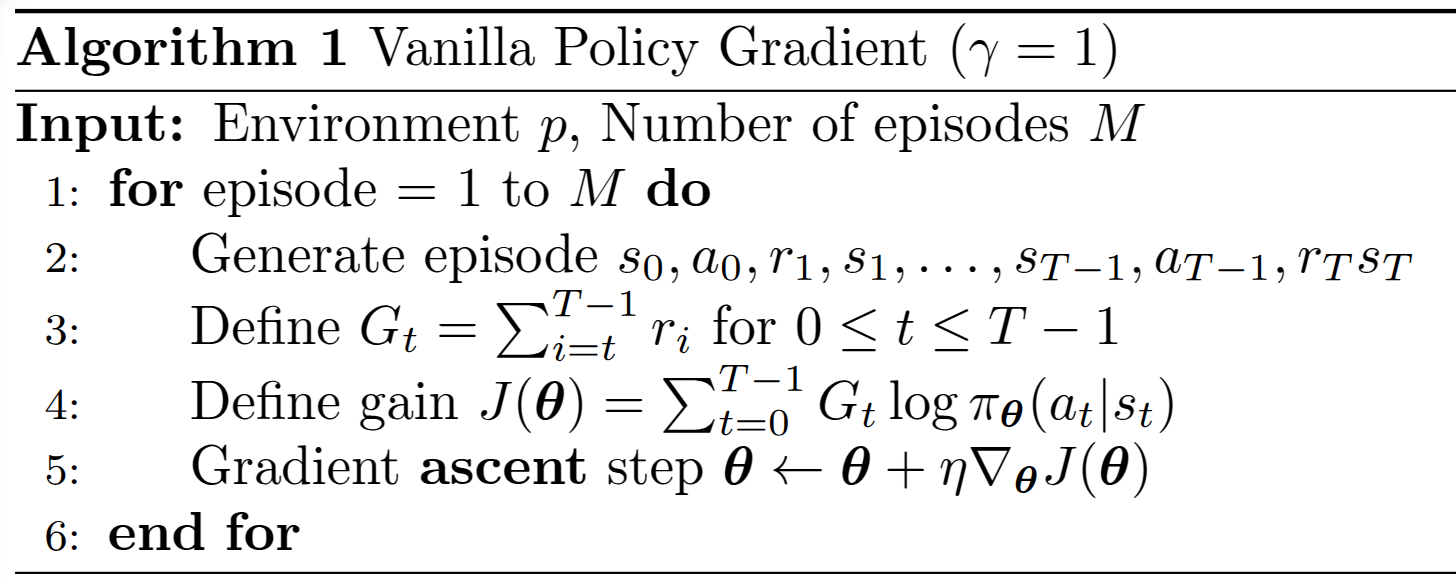
\includegraphics[width=1\linewidth]{img/vpg}
            % generated from algo.tex
		\label{fig:vpg}
	\end{figure}
%	\bs
VPG generates a trajectory, learns, then discards it, generates another.
\end{frame}


% \begin{frame}
%     \frametitle{REINFORCE with Reward-to-Go}
%     \textbf{Refined Policy Gradient:}
%     \begin{align*}
%         \nabla_{\bth} J(\bth) 
%         &= \Ex_{\tau \sim \pi_{\bth}} 
%         \left[ \sum_{t=0}^{\eplen - 1} \nabla_\bth \log \pi_\bth(a_t|s_t) \cdot G(\tau) \right] \\
%         &\textcolor{gray}{\text{(Full return version)}} \\
%         &= \Ex_{\tau \sim \pi_{\bth}} 
%         \left[ \sum_{t=0}^{\eplen - 1} \nabla_\bth \log \pi_\bth(a_t|s_t) \cdot G_t \right] \\
%         &\textcolor{gray}{\text{(Reward-to-go: unbiased and lower variance)}}
%     \end{align*}
%     \vspace{0.5em}
%     \textbf{Justification:} Only future rewards depend on $a_t$. Earlier rewards are unaffected, so including them adds noise.
% \end{frame}

\begin{frame}
    	\textbf{Clever trick 1: The future cannot affect the past}
    \begin{itemize}
        \item In REINFORCE, each $\log \pi_\bth(a_t|s_t)$ is multiplied by the full return $G(\tau)$.
        \item But $a_t$ cannot influence rewards that happened \textbf{before} it.
        \item \href{https://spinningup.openai.com/en/latest/spinningup/extra\_pg\_proof2.html}{Can be shown that}
        we can replace $G(\tau)$ with the \textbf{reward-to-go}:
        $$
        G_t := \sum_{t'=t+1}^{\eplen} r_{t'} = r_{t+1} + \ldots + r_{\eplen}
        $$
        which (in expectation) is the same as the Q-value $Q_{\pi_\bth}(s_t,a_t)$.
        \item This gives a lower-variance, unbiased estimator.

    \end{itemize}
    \begin{align*}
        %		\nabla_{\bth} J(\bth) &=
        %		\Ex_{\tau \sim \pi_{\bth}} 
        %		\left[ \nabla_\bth \sum_{k=t}^{\eplen} \log \pi_\bth(a_k|s_k) 
        %		\sum_{j = k}^{\eplen} R(s_j, a_j, s_{j+1}) \right] \\
        \nabla_{\bth} J(\bth) &=
        \Ex_{\tau \sim \pi_{\bth}} 
        \left[  \sum_{t=0}^{\eplen-1} \nabla_\bth \log \pi_\bth(a_t|s_t) \red{G(\tau)} \right]  \\
        &= \Ex_{\tau \sim \pi_{\bth}} 
        \left[ \sum_{t=0}^{\eplen - 1} \nabla_\bth \log \pi_\bth(a_t|s_t) \red{G_t} \right] \\
        &= \Ex_{\tau \sim \pi_{\bth}} 
        \left[ \sum_{t=0}^{\eplen-1} \nabla_\bth \log \pi_\bth(a_t|s_t) 
        \red{Q_{\pi_\bth}(s_t, a_t)} \right] 
        %	&= \Ex_{\tau \sim \pi_{\bth}} 
        %\left[ \nabla_\bth \sum_{k=t}^{\eplen} \log \pi_\bth(a_k|s_k) 
        %\hat{R}_t \right] 
     \end{align*}
\end{frame}


%\begin{frame}
%	\begin{figure}
%		\centering
%		\includegraphics[width=1\linewidth]{img/vpg_good}
%		\label{fig:vpggood}
%	\end{figure}
%%	\bs
%\end{frame}

%\subsection{Expected Grad-Log-Prob (EGLP) Lemma}
%\begin{frame}
%	\frametitle{Expected Grad-Log-Prob (EGLP) Lemma}
%	Let $\P_\bth$ be a parameterised probability distribution over random variable $x$.
%	Then
%	$$
%	\Ex_{x \sim \P_\bth}[\nabla_\bth \log \P_\bth(x)] = 0
%	$$
%	\pause
%	Proof:
%	\begin{align*}
%		\onslide<2->{& \sum_x \P_\bth(x) = 1 \\}
%		\onslide<3->{& \nabla_\bth \sum_x \P_\bth(x) = \nabla_\bth 1 = 0 \\}
%		\onslide<4->{& \nabla_\bth \sum_x \P_\bth(x) = 0 \\}
%		\onslide<5->{&\sum_x \nabla_\bth  \P_\bth(x) = 0}
%		\onslide<6->{\intertext{Apply log-derivative trick }}
%		\onslide<7->{&\sum_x  \P_\bth(x) \nabla_\bth  \P_\bth(x) = 0 \\}
%		\onslide<8->{& \Ex_{x \sim \P_\bth} [\nabla_\bth \log \P_\bth(x)] = 0}
%	\end{align*}
%\end{frame}

\subsection{Baseline Functions}
\begin{frame}
	\textbf{Theorem:} By the \href{https://spinningup.openai.com/en/latest/spinningup/rl\_intro3.html\#expected-grad-log-prob-lemma}{EGLP Lemma}, (i.e. math) we have 
	$$
	\Ex_{a_t \sim \pi_\bth}[\nabla_\bth \log \pi_\bth(a_t | s_t) b(s_t)] = 0
	$$
    for any \href{https://spinningup.openai.com/en/latest/spinningup/rl\_intro3.html\#baselines-in-policy-gradients}{baseline} function $b$ depending only on state. 
	\pause
	So, can add/subtract any such $b$ to decrease variance $\equiv$ speed up learning
	$$
	\nabla_{\bth} J(\bth) 
	= \Ex_{\tau \sim \pi_{\bth}} 
	\left[ \sum_{t=0}^{\eplen-1} \nabla_\bth \log \pi_\bth(a_t|s_t) 
	\bigg( Q_{\pi_\bth}(s_t, a_t)  \red{- b(s_t)} \bigg) \right] 
	$$
	\pause
	\textbf{Clever trick 2:}
	Choose $b(s_t) = \widehat{V}_\pi(s_t)$ as (some estimate of) the value function.
	\begin{align*}
%		\nabla_{\bth} J(\bth) 
%		&= \Ex_{\tau \sim \pi_{\bth}} 
%		\left[ \nabla_\bth \sum_{k=t}^{\eplen} \log \pi_\bth(a_k|s_k) 
%		\bigg( Q_{\pi_\bth}(s_k, a_k)  - V_{\pi_\bth}(s_k) \bigg) \right] \\
		\nabla_{\bth} J(\bth) &= \Ex_{\tau \sim \pi_{\bth}} 
		\left[  \sum_{t=0}^{\eplen-1} \nabla_\bth \log \pi_\bth(a_t|s_t) 
		A_{\pi_\bth}(s_t,a_t)  \right]
	\end{align*}
	where $\widehat{A}_\pi(s,a) := Q_\pi(s,a) - \widehat{V}_\pi(s)$ is the \textbf{advantage} function 
    \begin{itemize}
        \item how much
        better taking action $a$ is compared to sampling from $\pi(\cdot | s)$. 
        \item (assuming optimal value function) with no advantage $(A_\pi = 0)$, stop learning, $(\nabla_{\bth} J(\bth) =0)$.
    \end{itemize}
    
    
\end{frame}


\begin{frame}
    \frametitle{Aside: $n$-step update}
    Recall TD(0): $\widehat{V}_\pi(s_t)  \leftarrow \widehat{V}_\pi(s_t) + \alpha \delta_t$ where
    $$
    \delta_t \equiv \delta_{t:t+1} = r_{t+1} + \red{\gamma \widehat{V}_\pi(s_{t+1})} - \widehat{V}_\pi(s_t)
    $$
    \pause
    Why not include the information from two time-steps?
    $$ 
    \delta_{t:t+2} = r_{t+1} + \red{\gamma r_{t+2}  + \gamma^2 \widehat{V}_\pi(s_{t+2})} - \widehat{V}_\pi(s_t)
    $$
    \pause
    In general, we can perform $n$-step return updates:
    $$ 
    \delta_{t:t+n} = r_{t+1} + \red{\gamma r_{t+2}  + \ldots + \gamma^{n-1} r_{t+n}  + \gamma^{n} \widehat{V}_\pi(s_{t+n})} - \widehat{V}_\pi(s_t)
    $$
    \pause
    Or full rollout to the end of the episode (Monte Carlo (MC) update):
    $$
    \delta_{t:\eplen} = r_{t+1} + \red{\gamma r_{t+2} + \gamma^2 r_{t+3} + \ldots + \gamma^{\eplen-(t+1)} r_\eplen} - \widehat{V}_\pi(s_t)
    $$
    where $\eplen$ is the final time step of the episode.
    
\end{frame}

\subsection{Optimising for Advantage}

\begin{frame}
    \frametitle{Aside: $n$-step update}
    Complete return $G_t \equiv G_{t:T} = r_{t+1} + \gamma r_{t+2} + \ldots + \gamma^{T-t-1} r_T$.
    Can write approximations using $n$-step returns:
    $$
    G_{t:t+n} = r_{t+1} + \gamma r_{t+2} + \ldots + \gamma^{n-1} r_{t+n}  + \gamma^{n} \hat{V}_\pi(s_{t+n})
    $$
    \pause
    In TD(0), we use the single-step return:
    \begin{align*}
        \delta_t &= G_{t:t+1} - \hat{V}_\pi(s_t) \\
        G_{t:t+1} &= r_{t+1} + \gamma \hat{V}_\pi(s_{t+1}) 
    \end{align*}
    \pause
    Can now write $n$-step TD update as:
    $$
    \delta_{t:t+n} = G_{t:t+n} - \hat{V}_\pi(s_t)
    $$
    \pause
    Can be shown that $n$-step return $G_{t:t+n}$ are all valid targets for TD updates.
    \begin{itemize}
        \item Smaller $n$: Lower variance, higher bias
        \item Larger $n$: Higher variance, lower bias
        \item ...is there a way to get the benefits of both?
    \end{itemize}
\end{frame}

\begin{frame}
    \frametitle{Mixing updates}
    Can have any mixture of $n$-step returns as a valid target for TD updates. For example,
    $$
    \delta_{t} = \frac{G_{t:t+1} + G_{t:t+2}}{2} - \hat{V}_\pi(s_t)
    $$
    is a valid TD update (an average of 1-step and 2-step returns).
    
    \pause
    TD($\lambda$) mixes over all $n$-step returns, weighting\footnote{Note that $\sum_{n=0}^\infty \lambda^n = \frac{1}{1-\lambda}$, so we scale weighting by $1-\lambda$.}
    $G_{t:t+n}$ by weight $w_{n} \propto \lambda^{n}$
    $$
    \delta^\lambda_t = w_1 G_{t:t+1} + w_2 G_{t:t+2} + w_3 G_{t:t+3} + \ldots - \hat{V}_\pi(s_t) 
    $$
    The further forward in the future, the less weight it has.
    \pause
    % \frametitle{TD($\lambda$)}
    % Mix over all $n$-step updates, and decay 
    % them based on how far back in the past they are.
%     \begin{align*}
%    \frac{1}{1-\lambda} G^\lambda_t &:= \sum_{n=0}^\infty \lambda^n G_{t:t+n+1}  \\
%    & = G_{t:t+1} + \lambda G_{t:t+2} + \lambda^2 G_{t:t+3} + \ldots \\
%    &= r_{t+1} + \gamma \hat{V}_\pi(s_{t+1}) - \hat{V}_\pi(s_t) \\
%    &+ \lambda \left( r_{t+1} + \gamma r_{t+2} + \gamma^2 \hat{V}_\pi(s_{t+2}) - \hat{V}_\pi(s_t) \right) \\
%    &+ \lambda^2 \left( r_{t+1} + \gamma r_{t+2} + \gamma^2 r_{t+3} + \gamma^3 \hat{V}_\pi(s_{t+3}) - \hat{V}_\pi(s_t) \right) \\
%    &+ \ldots
%     \end{align*}
    \begin{block}{TD($\lambda$) update}
$$
    \delta^\lambda_t = G^\lambda_t - \hat{V}_\pi(s_t) \text{ where }  G^\lambda_t = (1-\lambda) \sum_{n=0}^\infty \lambda^n G_{t:t+n+1}
    $$
    \end{block}
    \pause
\textbf{Exercise:} Prove TD($\lambda$) for $\lambda = 0$ is TD(0), and that TD(1) is MC.

\end{frame}

\subsection{Eligibility Traces}
\begin{frame}
    \frametitle{Eligibility Traces}
    Because \href{https://davidstarsilver.wordpress.com/wp-content/uploads/2025/04/lecture-4-model-free-prediction-.pdf}{math} one can compute the TD($\lambda$) update rule 
    \begin{align*}
        \hat{V}_\pi(s_t)  &\leftarrow
        \hat{V}_\pi(s_t) + \alpha \delta^\lambda_t \\
        & \leftarrow  \hat{V}_\pi(s_t) + \alpha \left( (1-\lambda)  \left[ \sum_{n=0}^\infty \lambda^n G_{t:t+n+1}  \right] - \hat{V}_\pi(s_t) \right) \\
    \end{align*}
    very efficiently as
    \begin{align*}
        \hat{V}_\pi(s_t)  \leftarrow \hat{V}_\pi(s_t) + \alpha \delta_t E_t(s_t)
    \end{align*}
    where $E$ is the \textbf{eligibility trace}
    \begin{align*}
     E^0(s) &:= 0 \\
     E^t(s) &:= \gamma \lambda E^{t-1}(s) + \iver{s = s_t}
     \end{align*}
     and $\delta_t = G_{t:t+1} - \hat{V}_\pi(s_t)$
     is the standard 1-step TD error. We use this for PPO advantage $A_t$.
     
    \begin{figure}
        \centering
        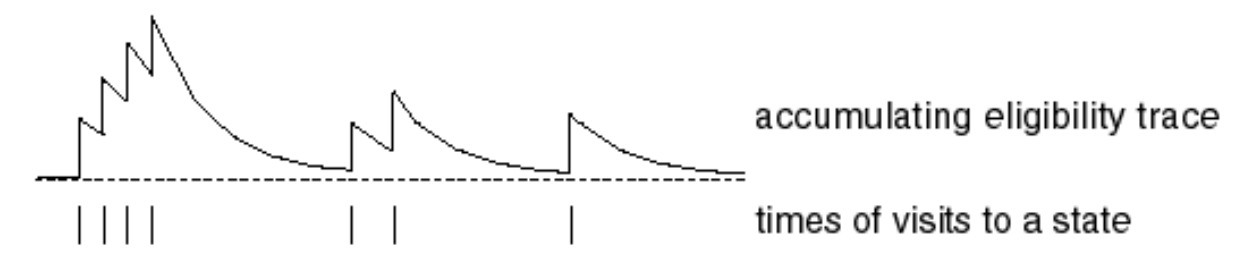
\includegraphics[width=0.5\linewidth]{img/eligibility.png}
    \end{figure}


    
    
%    \begin{block}{TD(0) update}
%        $$
%        \hat{V}_\pi(s_t)  \leftarrow
%        \hat{V}_\pi(s_t) + \alpha \left( r_{t+1} + \gamma \hat{V}_\pi(s_{t+1}) - \hat{V}_\pi(s_t) \right) 
%        $$
%    \end{block}
%    
%    \begin{itemize}
%        \item Only provides an update based on the most recent state $s_t$
%        \pause
%        \item What if the pivotal action was taken far in the past,
%        that lead to this desirable state?
%        \pause
%    \end{itemize}
%    
%    One solution is to keep track of the \textbf{Eligibility Trace}, the number of times a state has been visited, discounted
%    geometrically via a parameter $\lambda$, called the \textbf{trace decay}, and by $\gamma$, the \textbf{discount rate}.
%    \begin{align*}
%        E^0(s) &:= 0 \\
%        E^t(s) &:= \gamma \lambda E^{t-1}(s) + \iver{s = s_t}
%    \end{align*}
%    
%    \pause
%    
%    \textbf{Motivation:} States that are visited more often have more influence.
%    
%    The discounting allows for more recent visits to contribute more to the count than past visits (which may be valuable for
%    non-stationary environments.)
    
\end{frame}

\begin{frame}
    \frametitle{Actor-Critic VPG}
    Approximate advantage as $\hat{A}_t \equiv \hat{A}_{\pi_{\bth}}(s_t, a_t) = \hat{Q}_{\pi_\bth}(s_t, a_t) - \hat{V}_{\pi_\bth}(s_t)$.
    $$
    \nabla_\bth J(\bth) = \Ex_{\tau \sim \pi_{\bth}} 
    \left[ \sum_{t=0}^{\eplen-1} \nabla_\bth \log \pi_\bth(a_t|s_t) 
    \bigg( \hat{Q}_{\pi_\bth}(s_t, a_t) - \hat{V}_{\pi_\bth}(s_t) \bigg) \right]
    $$
    where:
    \pause
    \begin{itemize}
        \item Approx $Q_{\pi_\bth}$ using empirical return,
        $
        \hat{Q}_{\pi_\bth}(s_t, a_t) := G_{t} = \sum_{t'=t+1}^T r_{t'}
        $
        \pause
        \item Approx $V_{\pi_\bth}$ using \textbf{critic} network 
        $
        \hat{V}_{\pi_{\bth}}(s_t) := V_\pth(s_t)
        $ with parameters $\pth$
        \pause
        \item Approximate the expectation $\Ex_{\tau \sim \pi_{\bth}}$ by sampling $\hat{\Ex}$
        \pause
        $$
        \nabla_\bth J(\bth) \approx \hat{\Ex}_{\tau \sim \pi_{\bth}} 
        \left[ \sum_{t=0}^{\eplen-1} \nabla_\bth \log \pi_\bth(a_t|s_t) 
        \bigg( G_t - \hat{V}_{\pi_\bth}(s_t) \bigg) \right]
        $$
        \item $\pi_\bth$ is the \textbf{actor} and $V_\pth$ is the \textbf{critic}.
    \end{itemize}
    \end{frame}
    
    \begin{frame}
        \frametitle{Critic Loss}
        The critic is simply trained against the returns from the environment. We define
        the \textbf{value function} loss or \textbf{critic loss} as 
        \begin{align*}
        L^{VF}(\pth) &=  \hat{\mathbb{E}}_t [V_\pth(s_t) - G^\lambda_t]^2 \\
        % &= \frac{1}{|\mathcal{B}|} \sum_{b=1}^{|\mathcal{B}|} 
        % \left[ \sum_{t=1}^{\eplen} \left( V_\pth(s^b_t) - V^\text{target}_t \right)^2 \right]
        \end{align*}
        % over a batch  $\mathcal{B} = \{\tau^1, \tau^2, \ldots \tau^{|\mathcal{B}|} \}$
        % of episodes with trajectories $\tau^b = s^b_{0}, a^b_0, r^b_1, s^b_1, \ldots, s^b_{\eplen}$ and returns $G^b_t = \sum_{k=t+1}^T r^b_k$.
        where $G^\lambda_t$ is the target for TD($\lambda$) introduced for eligibility traces.
        
        
    \end{frame}

\begin{frame}
    \frametitle{PPO: The big picture}
    PPO is just Actor-Critic VPG with a bag of tricks/heuristics on top:
    \begin{itemize}
        \item Use importance sampling to allow off-policy training.
        \item Clip the importance sampling ratio so new policy doesn't drift too far.
        \item Use Actor-Critic method for stability:
        \begin{itemize}
            \item Actor chooses the actions
            \item Critic learns the value of states, and provides feedback to the actor. 
        \end{itemize}
        \item Add an entropy bonus to prevent the policy converging on deterministic too fast.
    \end{itemize}
    \pause
    Q: Is the bag of tricks well motivated/principled? 
    \pause
    
    A: Somewhat? Importance sampling is principled, clipping is kind of hacky, and entropy bonus
    really feels like an afterthought, but it works!
\end{frame}





%\begin{frame}
%    \frametitle{Aside: Generalised Advantage Estimation}
%    
%    Penalising TD updates using the eligibility trace, this gives us the update rule for TD($\lambda$). On timestep $t$, perform update
%    \begin{align*}
%        \forall s \in \mathcal{S}, \hat{V}_\pi(s) & \leftarrow \hat{V}_\pi(s) + \alpha \red{E^t(s)}  \left( r_{t+1} + \gamma \hat{V}_\pi(s_{t+1}) - \hat{V}_\pi(s_t) \right)  \\
%    \end{align*}
%    Above expression can be unrolled for the advantage function (exercise to reader.) 
%    $$
%    \hat{A}_t = \delta_t +(\gamma \lambda)\delta_{t+1} + \ldots + 
%    (\gamma \lambda)^{T-(t+1)} \delta_{T-1}
%    $$
%    where
%    $\delta_t = r_{t+1} + \gamma V(s_{t+1}) - V(s_t)$.
%    
%    We use this for the advantage function for PPO, so that TD-errors from the past also contribute.
%\end{frame}







%\begin{frame}
%	\frametitle{\red{WARNING}}
%	
%	\red{Everything beyond this point, I am less certain about.
%	Where I make my best guess, or am uncertain, I mark it with \bs.}
%\end{frame}
%
%\begin{frame}
%	\frametitle{Empirical Policy Gradient}
%	\textbf{Note:} Police gradient uses gradient \textbf{ascent}, so we actually
%	\textbf{maximise} loss!
%	\pause
%	\begin{itemize}
%		\item Don't blame me, the PPO paper use this convention too!
%	\end{itemize}
%	\pause
%	Define policy gradient ``loss'' (gain?) 
%	$$
%	L^{PG}(\bth) = \hat{\Ex} \left[ \sum_{k=t}^{\eplen} \log \pi_\bth(a_k|s_k) 
%	A_{\pi_\bth}(s_t,a_t)\right]
%	$$
%	where $\hat{\Ex}$ indicates the expectation is approximated by a batch of samples,
%	and $\hat{A}(s_t,a_t) = \hat{Q}(s_t,a_t) - \hat{V}_\pth(s_t)$, where
%	\pause
%	\begin{itemize}
%		\item $Q(s_t,a_t) = \sum_{k=t}^{\eplen} R(s_t, a_t, s_{t+1})$ Q-value computed using
%		empirical return \bs
%		\pause
%		\item $\hat{V}_\pth(s_t)$ computed using critic network
%		\pause
%		\item Note that $\hat{A}(s_t,a_t)$ has no dependance on $\bth$.
%		\pause
%		\item However, this leads to destructively large policy updates
%		\pause
%	\end{itemize}
%\end{frame}
%
%\subsection{Importance Sampling}
%\begin{frame}
%	\frametitle{Importance Sampling}
%	\textbf{Main Idea:} Use samples from one distribution to estimate the expected 
%	value of a function under a different distribution.
%	
%	In RL, policy $\pi$ being learned about is \textbf{target policy} 
%	(usually $\pi_*$), policy generating behaviour 
%	$\beta$ is \textbf{behaviour policy}.
%	\pause 
%	
%	\textbf{On-Policy:} target=behaviour
%	
%	\begin{itemize}
%		\pause 
%		\item SARSA: Target policy $\pi^\varepsilon_*$, behaviour policy $\pi^\varepsilon_*$
%		(on-policy)
%		\pause 
%		\item Q-Learning:  Target policy $\pi_*$, behaviour policy $\pi^\varepsilon_*$ (off-policy)
%	\end{itemize}
%	\pause 
%	If $\pi$ is very different from $\beta$, high variance,
%	bad learning.
%\end{frame}
%
%\begin{frame}
%	\frametitle{Importance Sampling}
%	
%	Given starting state $s_t$, the probability of a particular state-action trajectory
%	from timestep $t$ to $\eplen$
%	$$
%	\tau = a_t, s_{t+1}, a_{t+1}, s_{t+2}, a_{t+2}, \ldots, a_{\eplen-1}, s_{\eplen}
%	$$
%	is
%	\begin{align*}
%		\text{Pr}(\tau | s_t, a_{t,\eplen-1} \sim \pi)
%		&= \pi(a_t|s_t) T(s_{t+1} | s_t, a_t) \pi(a_{t+1} | s_{t+1}) \ldots
%		T(s_{\eplen} | s_{\eplen-1}, a_{\eplen-1}) \\
%		&= \prod_{k=t}^{\eplen-1} \pi(a_k | s_k) T(s_{k+1} | s_k, a_k)
%	\end{align*}
%	\pause
%	\textbf{Importance-sampling ratio:} $\rho_{t:\eplen-1}$ The ratio of the likelihood of the trajectory
%	under target and behaviour policies.
%	$$
%	\rho_{t:\eplen-1} = \frac{\prod_{k=t} \pi(a_k | s_k) T(s_{k+1} | s_k, a_k)}
%	{\prod_{k=t} \beta(a_k | s_k) T(s_{k+1} | s_k, a_k)}
%	= \frac{\prod_{k=t} \pi(a_k | s_k)}
%	{\prod_{k=t} \beta(a_k | s_k) }
%	$$
%	\begin{itemize}
%		\item No dependancy on environment distribution $T$!
%	\end{itemize}
%\end{frame}
%
%\begin{frame}
%	\frametitle{Importance Sampling}
%	Want to estimate $V_\pi$, but only have returns $G^\beta_t$  
%	obtained from $\beta$. $G^\beta_t$ has the wrong expectation
%	$$
%	\Ex[G^\beta_t | s_t = s] = V_{\beta}(s)
%	$$
%	\pause
%	Transform with the importance sampling ratio!
%	$$
%	\Ex[\rho_{t:\eplen-1}G^\beta_t | s_t = s] = V_{\pi}(s)
%	$$
%	\pause
%	(\bs) During policy gradient, data is sampled from $\pi_{\bth_{old}}$, but target
%	is $\pi_\bth$, so we would rather optimise
%	$$
%	\hat{\Ex} \left[ \frac{\pi_{\bth}(a_t | s_t)}{\pi_{\bth_{old}}(a_t | s_t)}\hat{A}(s_t,a_t) \right]
%	$$ 
%	called the \textbf{surrogate} objective.
%\end{frame}

% \begin{frame}
%     \frametitle{\href{https://arxiv.org/abs/1502.05477}{Trust Region Policy Optimisation}}
%     \begin{itemize}
%         \item We keep $\bth_{\text{old}}$, an old set of the parameters $\bth$ to compare against.
%         \pause
%         \item Let $r_t(\bth)$ denote the \textbf{probability ratio} $r_t(\bth) = \frac{\pi_\bth(a_t | s_t)}{\pi_{\bth_{\text{old}}}(a_t | s_t)}$, so $r_t(\bth_{\text{old}}) = 1$. 
%         \begin{itemize}
%             \item Don't confuse probability ratio $r_t(\bth)$ with reward $r_t$!
%         \end{itemize}
%         \pause
%         TRPO maximizes the \textit{conservative policy iteration} (CPI) joy
        
%         $$
%         J^{CPI}(\bth) = \hat{\mathbb{E}}_t \left[ \frac{\pi_\bth(a_t | s_t)}{\pi_{\bth_{\text{old}}}(a_t | s_t)} \hat{A}_t \right] = \hat{\mathbb{E}}_t \left[ r_t(\bth) \hat{A}_t \right].
%         $$
%         	subject to the constraint 
%         $$
%         \hat{\Ex}_t \bigg[ \text{KL}[\pi_{\bth_\text{old}}(\cdot | s_t)\; ||\; 
%         \pi_\bth(\cdot | s_t)] \bigg] \leq \delta 
%         $$
%         to avoid $\pi_\bth$ changing too much.
%         \pause
%     \item \textbf{Intuition:} If the advantage $\hat{A}_{\pi_\bth}(s,a) > 0$, we
%     want to put more probability mass on action $a$ given state $s$, i.e.
%     make $\frac{\pi_\bth(a | s)}{\pi_{\bth_{\text{old}}}(a | s)} > 1$.
%     \pause
%     \item PPO improves on this by clipping the change directly rather than constrained optimisation.
%        \pause
%     \item \textbf{Note:} We cheat here: To avoid having two networks, we store $\log \pi(a_t | s_t)$ at the time when $a_t$ was sampled, and then use this as our value for $\pi_{\bth_{\text{old}}}$.
% \end{itemize}

% \end{frame}

%\begin{frame}
%	\frametitle{Justifying the surrogate objective}
%	\begin{itemize}
%		\item Take $L^{PG}(\bth)$, and subtract out $\log \pi_{\bth_{old}}(a_t|s_t) \hat{A}_t(s_t,a_t)$ (no dependence on $\bth$, maximising $\bth$ is unchanged) 
%		\pause
%		\begin{align*}
%			\onslide<2->{& \argmax_\bth L^{PG}(\bth)\\ 
%				&= \argmax_{\bth} \hat{\Ex} \left[ \sum_{k=t}^{\eplen} \log \pi_\bth(a_k|s_k) 
%				A_{\pi_\bth}(s_t,a_t)
%				-
%				\log \pi_{\bth_{old}}(a_t|s_t) \hat{A}_t(s_t,a_t)\right] \\}
%			\onslide<3->{&= \argmax_{\bth} \hat{\Ex} \left[
%				\sum_{k=t}^{\eplen} \log \frac{\pi_\bth(a_k|s_k)}{\pi_{\bth_{old}}(a_k|s_k)} 
%				\hat{A}_{\pi_\bth}(s_t,a_t)
%				\right]}
%			\onslide<4->{\intertext{$\log$ is monotonic/Jensens theorem/idk \bs}}
%			\onslide<5->{&= \argmax_{\bth} \hat{\Ex} \left[
%				\sum_{k=t}^{\eplen} \frac{\pi_\bth(a_k|s_k)}{\pi_{\bth_{old}}(a_k|s_k)} 
%				\hat{A}_{\pi_\bth}(s_t,a_t)
%				\right]}
%		\end{align*}
%		\onslide<6->{
%			\begin{tikzpicture}[remember picture,overlay]
%				\node [opacity=0.3,rotate=45,scale=10] at (current page.center) {\bs};
%		\end{tikzpicture}}
%	\end{itemize}
%\end{frame}


%\begin{frame}
%	\frametitle{Clip Objective}
%    \begin{align*}
%    J^{CLIP}(\bth) &= \hat{\mathbb{E}}_t \left[
%    \min(r_t(\bth) \hat{A}_t, \text{clip}(r_t(\bth), 1-\eps, 1+\eps)\hat{A}_t)
%    \right] \\
%    &= \hat{\mathbb{E}}_t \left[
%    \min(J^{CPI}(\bth), \text{clip}(r_t(\bth), 1-\eps, 1+\eps)\hat{A}_t)
%    \right] \\
%    \end{align*}
%    \textbf{Intuition:} Clip the probability ratio $r_t(\bth)$ to interval $[1-\eps, 1+\eps]$.
%    Then, take the minimum of clipped and unclipped objective, as a pessimistic bound.
%    
%\end{frame}
%


\section{Proximal Policy Optimisation (PPO)}
%\textit{
%\subsection{Trust Region Policy Optimisation (TRPO)}
%\begin{frame}
%	\frametitle{Trust Region Policy Optimisation (TRPO)}
%	(Drop summations, write $\hat{A}_t \equiv \hat{A}(s_t,a_t)$ for brevity).\\
%	The goal is maximisation of $L^{CPI}(\bth)$ w.r.t $\bth$ defined as
%	$$
%	L^{CPI}(\bth) = \Ex \left[ 
%	\frac{\pi_\bth(a_t | s_t)}{\pi_{\bth_\text{old}}(a_t | s_t)} \hat{A}_t \right]
%	$$
%	subject to the constraint 
%	$$
%	\hat{\Ex} \bigg[ \text{KL}[\pi_{\bth_\text{old}}(\cdot | s_t)\; ||\; 
%	\pi_\bth(\cdot | s_t)] \bigg] \leq \delta 
%	$$
%	to avoid the two distributions changing too much. \\
%	\pause
%	Here, $\text{KL}(p||q) := \sum_x p(x) \log \frac{p(x)}{q(x)}$ is the 
%	\textbf{Kullback-Liebler divergence}, or KL-divergence, that measures
%	the ``distance'' between two probability distributions.
%	\pause
%	Constrained optimisation is problematic to deal with, but unconstrained
%	optimisation with a KL-penalty
%	$$
%	\underset{\bth}{\text{maximise}}
%	\Ex \left[ \frac{\pi_\bth(a_t | s_t)}{\pi_{\bth_\text{old}}(a_t | s_t)} 
%	\hat{A}_t - \beta \text{KL}[\pi_{\bth_\text{old}}(\cdot | s_t)\; ||\; 
%	\pi_\bth(\cdot | s_t)]  \right]
%	$$
%	requires an additional hyperparameter $\beta$. Via experimentation, could not find
%	a single $\beta$ suitable for many different environments.
%\end{frame}
%}
\subsection{Importance Sampling}
\begin{frame}
    \frametitle{Importance Sampling}
    Recall VPG Joy estimator:
    $$
    J(\bth) \approx \hat{\Ex}_{\tau \sim \pi_{\bth}} 
    \left[ \sum_{t=0}^{\eplen-1} \log \pi_\bth(a_t|s_t) 
    \hat{A}_t \right]
    $$
    \begin{itemize}
        \item Inefficient to generate trajectories and then learn one at a time.
        \item Sample lots of trajectories, and then learn from them (perhaps many times).
        \item But during learning, data generated from $\pi_{\bth_{old}}$, but policy drifts to $\pi_\bth$.
        $$
        J(\bth) \not\approx \hat{\Ex}_{\tau \sim \pi_{\bth_{old}}} 
        \left[ \sum_{t=0}^{\eplen-1} \log \pi_\bth(a_t|s_t) 
        \hat{A}_t \right]
        $$
        \item VPG is an on-policy method, so we can't use it.
        \item We have $\tau \sim \pi_{\bth_{old}}$, but we need $\tau \sim \pi_\bth$.
    \end{itemize}
\end{frame}

\begin{frame}
    \frametitle{Importance Sampling}
    \begin{block}{Importance Sampling}
        Idea: Want to estimate $\Ex_{x \sim p}[f(x)]$ using samples from $q$.
        \begin{align}
        \label{eq:is}
        \Ex_{x \sim p}[f(x)] = \Ex_{x \sim q} \left[ \frac{p(x)}{q(x)} f(x) \right]
        \end{align}
    \end{block}
\end{frame}

\begin{frame}
    \frametitle{Importance Sampling}
    We can log the probabilities $\pi_{\bth_{old}}$ that were used to generate the trajectories:
    \begin{align*}
        \nabla J(\bth) &\approx \onslide<1->{\hat{\Ex}_{\tau \sim \pi_{\bth}} 
        \left[ \sum_{t=0}^{\eplen-1} \nabla_\bth \log \pi_\bth(a_t|s_t) 
        \hat{A}_t \right]} 
        \onslide<2->{=\hat{\Ex}_{\tau \sim \pi_{\bth}}  
        \left[ \sum_{t=0}^{\eplen-1} \frac{\nabla_\bth \pi_\bth(a_t|s_t)}{\pi_{\bth}(a_t|s_t)} 
        \hat{A}_t \right]} \\
        & \onslide<3->{=\hat{\Ex}_{\tau \sim \red{\pi_{\bth_{old}}}}
        \left[ \frac{P(\tau | \pi_{\bth})}{P(\tau | \red{\pi_{\bth_{old}}})} \sum_{t=0}^{\eplen-1}  
        \frac{\nabla_\bth \pi_\bth(a_t|s_t)}{\pi_{\bth}(a_t|s_t)} \hat{A}_t \right]} \\
        &\onslide<4->{\approx \hat{\Ex}_{\tau \sim \red{\pi_{\bth_{old}}}} 
        \left[ \sum_{t=0}^{\eplen-1} \frac{\cancel{\pi_\bth(a_t|s_t)}}{\red{\pi_{\bth_{old}}}(a_t|s_t)} 
        \frac{\nabla_\bth \pi_\bth(a_t|s_t)}{\cancel{\pi_{\bth}(a_t|s_t)}} \hat{A}_t \right]} \\
        & \onslide<5->{=\hat{\Ex}_{\tau \sim \red{\pi_{\bth_{old}}}} 
        \left[ \sum_{t=0}^{\eplen-1} \frac{\nabla_\bth \pi_\bth(a_t|s_t)}{\red{\pi_{\bth_{old}}}(a_t|s_t)} 
        \hat{A}_t \right]} \onslide<5->{=\hat{\Ex}_{\tau \sim \red{\pi_{\bth_{old}}}} 
        \left[ \sum_{t=0}^{\eplen-1} \nabla_\bth \red{r_t(\bth)} \hat{A}_t \right]}
    \end{align*}
    where $\red{r_t(\bth)} = \frac{\pi_\bth(a_t|s_t)}{\red{\pi_{\bth_{old}}}(a_t|s_t)}$ is the \emph{importance ratio}.
    Note that $r_t(\bth_{\text{old}}) = 1$.
\end{frame}

\begin{frame}
    \frametitle{PPO Clip Joy}
    $$J(\bth) = \hat{\Ex}_{\tau \sim \pi_{\bth_{old}}} 
    \left[ \sum_{t=0}^{\eplen-1} r_t(\bth) \hat{A}_t \right]$$
    \begin{itemize}
        \item Last dirty hack: try to make only a small update 
        by clipping $r_t(\bth) = \frac{\pi_{\bth}(a_t|s_t)}{\pi_{\bth_{old}}(a_t|s_t)}$ 
        to be in the range $[1-\epsilon,1+\epsilon]$.
        $$
        J^{small}(\bth) = \hat{\Ex}_{\tau \sim \pi_{\bth_{old}}} 
        \left[ \sum_{t=0}^{\eplen-1} \text{clip}(r_t(\bth), 1-\epsilon, 1+\epsilon) \hat{A}_t \right]
        $$
        \pause
        \item Be conservative, and take smaller of the clipped and unclipped objective 
        to get a lower bound on the unclipped objective.
        See \href{https://arxiv.org/pdf/1707.06347.pdf}{Section 3 of PPO paper}.
    \end{itemize}
    \begin{block}{PPO Clip Joy}
        \vspace{-0.4cm}
        \begin{align*}
        J^{CLIP}(\bth) &= \hat{\mathbb{E}}_t
	\left[ \sum_{t=0}^{\eplen-1}
	\min \big( r_t(\bth) \hat{A}_t, 
	\text{clip}(r_t(\bth), 1-\epsilon, 1+\epsilon) \hat{A}_t \big)
	\right]
   	\end{align*}
    \end{block}
	for \textbf{magic number} $\epsilon = 0.2$.
    
 
\end{frame}


\begin{frame}
    \frametitle{Entropy Bonus}
    \begin{itemize}
    \item We also add an \textbf{entropy bonus} to incentivise exploration
    by increasing the \textbf{entropy} of the distribution. The entropy
    $H_\pi(s)$ of a policy $\pi$ in state $s$ is defined as
    $$
    H_\pi(s) = \sum_{\substack{a \in \mathcal{A} \\ \pi(a|s) > 0}} \pi(a|s) \log \frac{1}{\pi(a|s)}
    $$ 
    \item Entropy can be thought of as a measure of how ``random'' the distribution is,
     \item Entropy bounded by $0 \leq H_\pi \leq \log |\mathcal{A}|$. 
     \item Min entropy of 0 means a deterministic policy (all the probability mass on one output). 
     \begin{itemize}
        \item Can also log $H_\pi(s)$ during training. If it crashes to zero, model probably got stuck.
     \end{itemize}
     \item Max entropy of $\log |\mathcal{A}|$ means the policy is uniformly guessing at random.
    \end{itemize}
\end{frame}

\begin{frame}
    \frametitle{Entropy Bonus}
    In practice, entropy bonus is computed as an average:
    \begin{align*}
    J^H(\bth) &:=  \hat{\mathbb{E}}_t \left[ H_{\pi_{\bth}}(s_t)
    \right] \\
    &= \frac{1}{|\mathcal{B}|} \sum_{b=1}^{|\mathcal{B}|} 
    \sum_{t=0}^{T-1}   \left[ \sum_{a \in \mathcal{A}} \pi_\bth(a|s^b_t) 
    \log \frac{1}{\pi_{\bth}(a|s^b_t)} \right]
    \end{align*}
    
    \textbf{Note:} We sum over all actions $a$, no dependency on the actual
    action $a_t$ taken!
\end{frame}


% \begin{frame}
%     \begin{figure}
%         \begin{tikzpicture}
%             \begin{axis}[
%                 xlabel={$p$},
%                 ylabel={$H(X)$},
%                 xmin=0, xmax=1,
%                 ymin=0, ymax=1,
%                 xtick={0,0.5,1},
%                 ytick={0,1},
%                 axis lines=middle,
%                 enlargelimits=true,
%                 clip=false,
%                 grid=major,
%                 legend style={at={(0.5,-0.2)},anchor=north},
%                 legend cell align=left,
%                 ]
%                 \addplot[blue,domain=0:1,samples=100] {-x*log2(x)-(1-x)*log2(1-x)};
%                 \legend{$H(X)=-p\log_2 p-(1-p)\log_2(1-p)$}
%             \end{axis}
%         \end{tikzpicture}
%         \caption{The entropy of a policy over two actions $\mathcal{A} = \{a_1, a_2\}$ 
%             with $\pi(a_1|s) = p$.}
%     \end{figure}
% \end{frame}



\begin{frame}
    \frametitle{PPO at long last!}
   \begin{block}{PPO Loss/Gain functions ($\sum$ and $\Ex$ suppressed)}
        \vspace{-0.5cm}
        \begin{align*}
            J_t^{CLIP}(\bth) &= 
            \min(r_t(\bth) \hat{A}_t, 
            \text{clip}(r_t(\bth), 1-\epsilon, 1+\epsilon) \hat{A}_t )
            & \text{[clip joy]} \\
            L_t^{VF}(\pth) &= (V_\pth(s_t) - G^\lambda_t)^2 & \text{[critic loss]}\\
            J_t^H(\bth) &= H_{\pi_{\bth}}(s_t) & \text{[entropy joy]}
        \end{align*}
   \end{block}

    
    Combine them all, with magic numbers $c_{VF} \approx 0.5$, $c_{H} = 0.01$, and $\epsilon = 0.2$.
    \begin{block}{PPO Objective}
        $$
    J^{PPO}(\bth, \pth)
    = \hat{\Ex}_t[J_t^{CLIP}(\bth) - c_{VF} L_t^{VF}(\pth) + c_{H} J_t^H(\bth)]
    $$
    \end{block}
    Maximise $J^{PPO}(\bth, \pth)$ with respect to policy 
    parameters $\bth$ and critic parameters $\pth$.
\end{frame}

\begin{frame}
    \begin{figure}
        \centering
        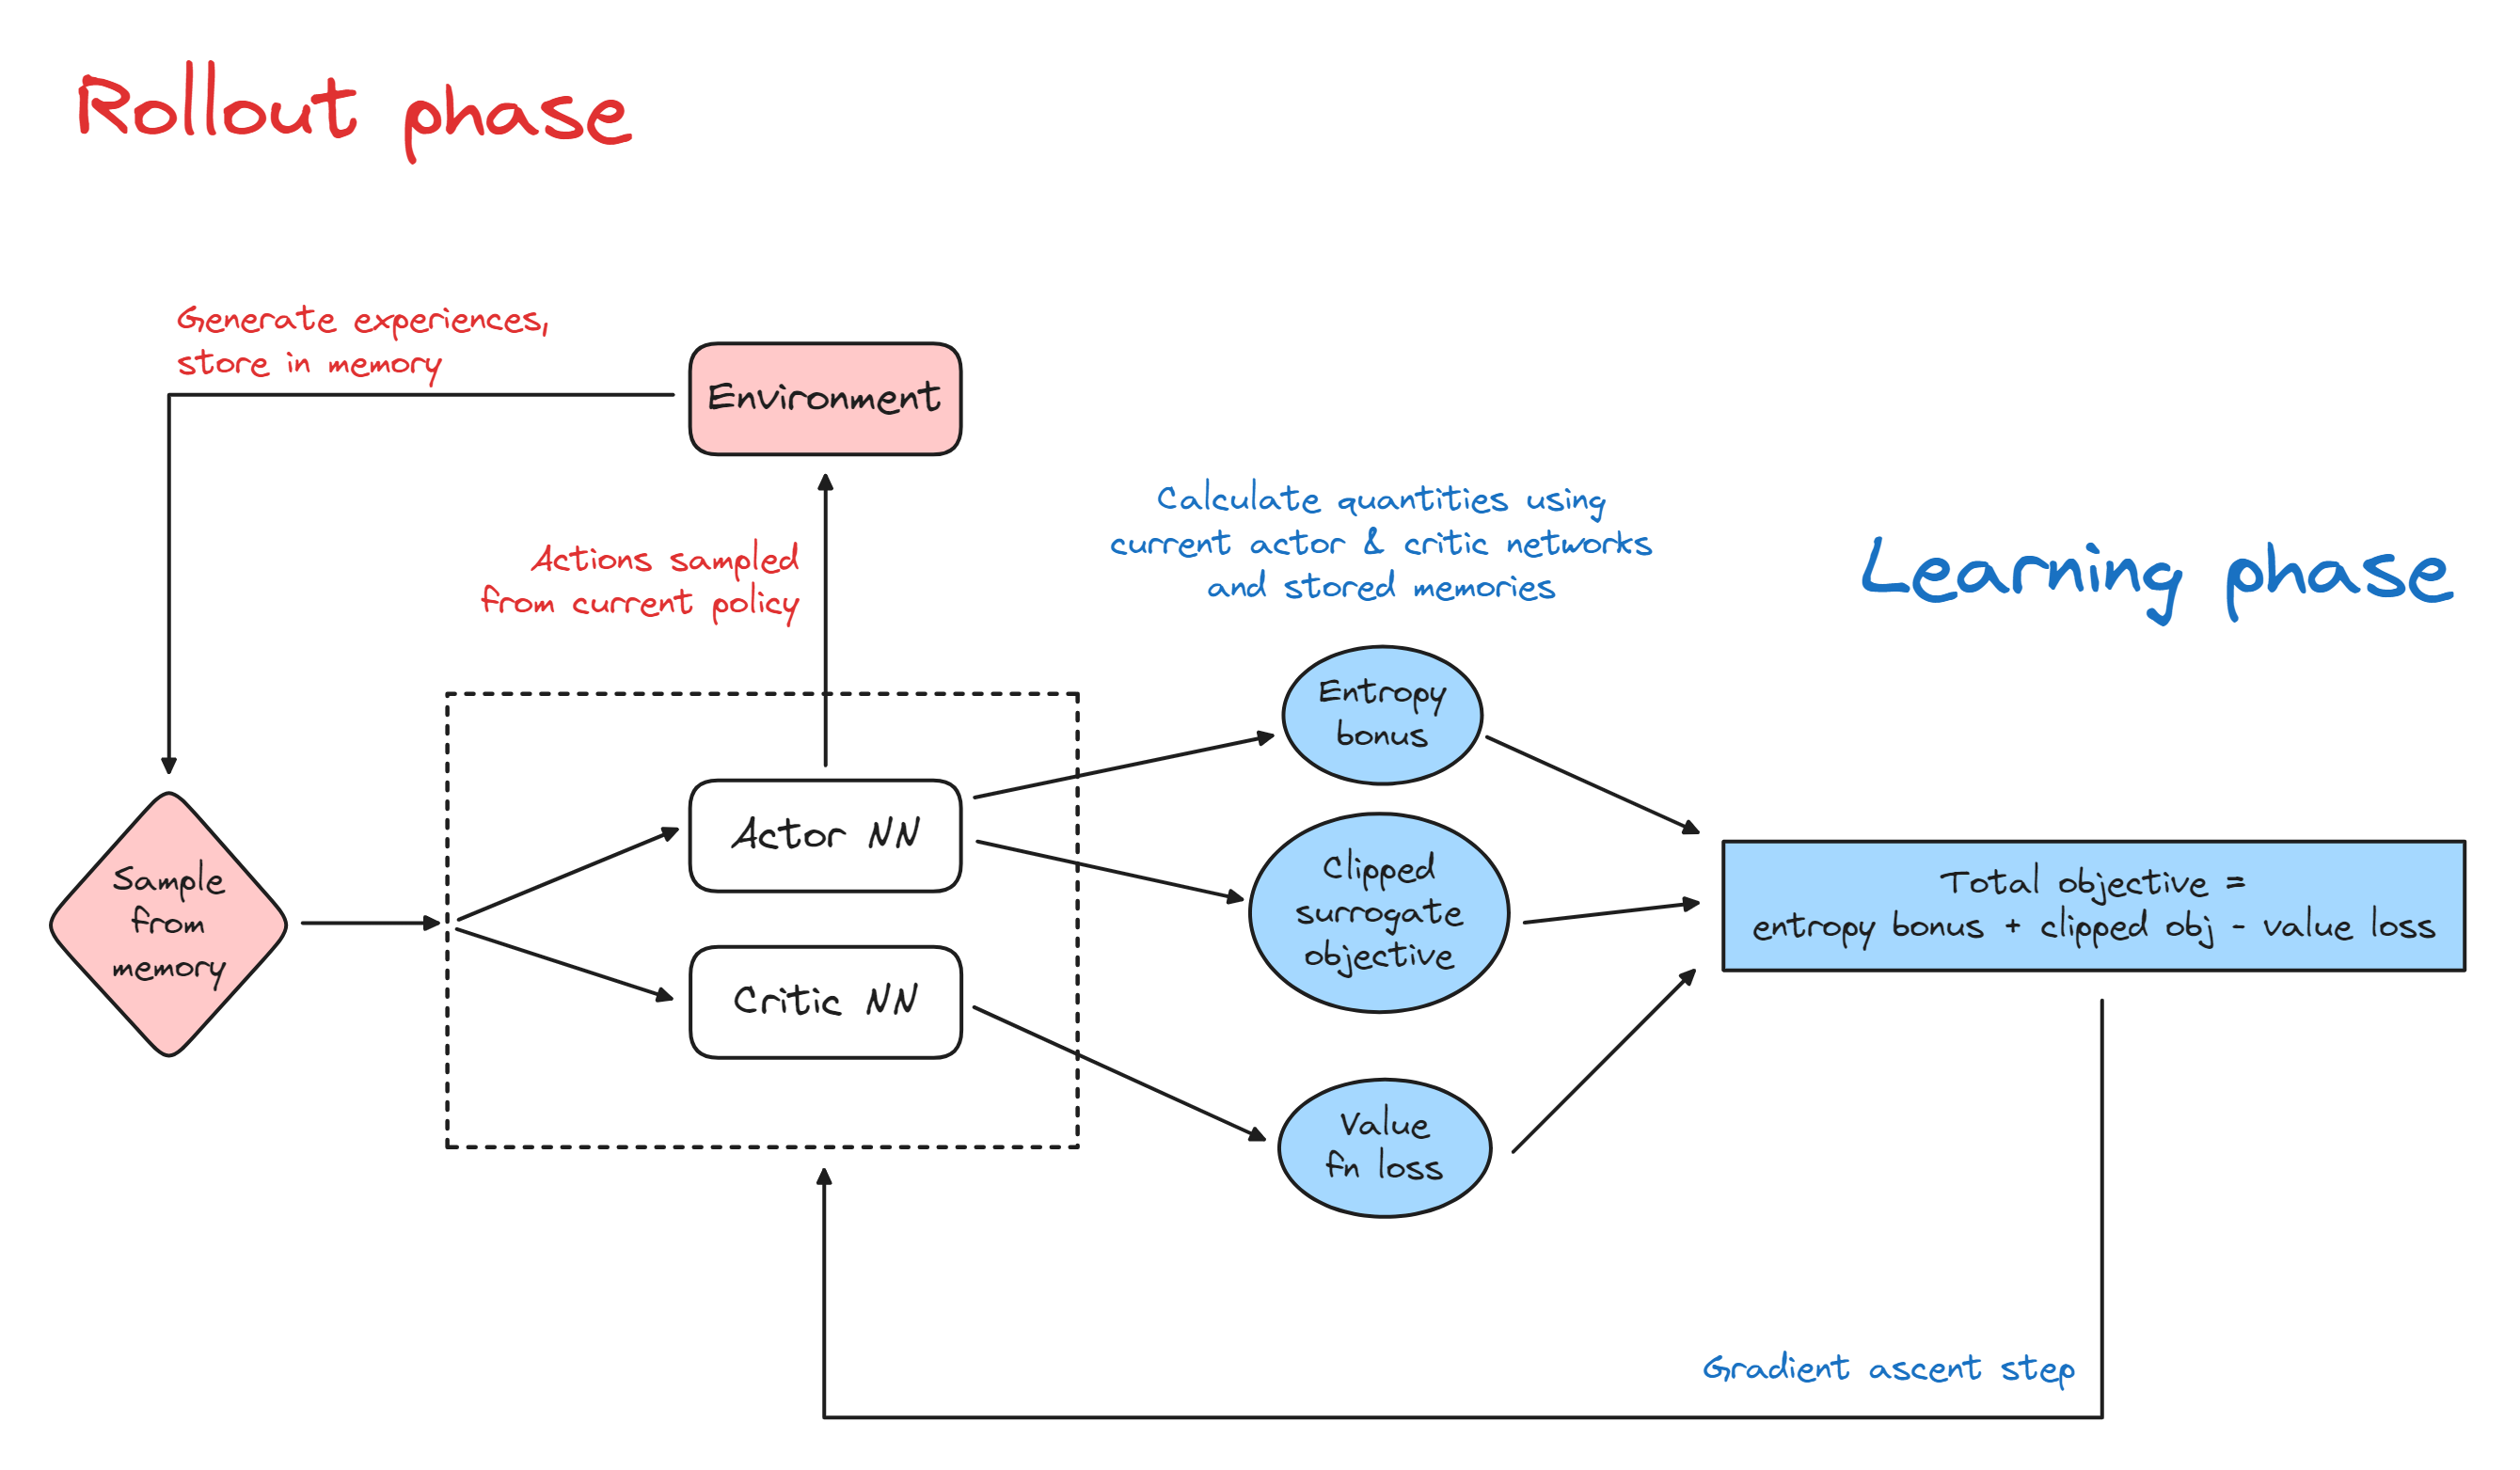
\includegraphics[width=\linewidth]{img/ppo_loop.png}
        \label{fig:ppoloop}
    \end{figure}
    
\end{frame}

%\begin{frame}
%    \Huge
%    \red{Machines get reset tomorrow for RLHF day!
%    Backup your stuff!}
%    \normalsize
%    
%\end{frame}
 

% \begin{frame}
% 	\frametitle{References}
	
% 	\begin{itemize}
% 		\item Sutton and Barto, Reinforcement Learning: An Introduction \url{http://incompleteideas.net/book/the-book-2nd.html}
% 		\item OpenAI Intro to Policy Optimisation \url{https://spinningup.openai.com/en/latest/spinningup/rl_intro3.html}
% 		\item PPO Paper
% 		\url{https://arxiv.org/pdf/1707.06347.pdf}
% 		\item Generalised Advantage Estimation
% 		\url{https://arxiv.org/pdf/1506.02438.pdf}
% 		\item \bs
% 	\end{itemize}
% \end{frame}

% \begin{frame}
% \frametitle{References}

% \begin{itemize}
% 	\item Sutton and Barto, Reinforcement Learning: An Introduction \url{http://incompleteideas.net/book/the-book-2nd.html}
% 		\item Yan LeCun's cake analogy, NeurIPS 2016,\url{https://www.youtube.com/watch?v=Ount2Y4qxQo&t=1072s}
% 	\item Jay Bailey's DQN Distillation \url{https://www.lesswrong.com/posts/kyvCNgx9oAwJCuevo/deep-q-networks-explained}
% 	\item Playing Atari with Deep Reinforcement Learning
% 	\url{https://www.cs.toronto.edu/~vmnih/docs/dqn.pdf}
% 	\item Human-level control through deep reinforcement learning
% 	\url{https://www.nature.com/articles/nature14236}
% 	\item Rainbow DQN \url{https://arxiv.org/abs/1710.02298}
% \end{itemize}
% \end{frame}



% \begin{frame}
% \frametitle{Robins-Monro Convergence conditions}

% The Robins-Monro convergence conditions are properties of the learning rate that
% are usually required in most proofs to ensure convergence.

% Let $\alpha_t$ denote the learning rate at time $t$. Then the conditions are

% $$
% \sum_{t=1}^\infty \alpha_t = \infty \text{ and } \sum_{t=1}^\infty \alpha_t^2 < \infty
% $$

% Intuitively, the first condition ensures that the steps are large enough to eventually overcome
% any initial conditions/random fluctuations, and the second condition ensures that eventually the 
% steps become small enough to ensure convergence.
% \pause 

% An example of such a learning rate would be $\alpha_t = 1/t$.

% Note that the usual method of choosing $\forall t, \alpha_t = \alpha \in \mathbb{R}$ 
% fails the RM conditions.
% \end{frame}


\end{document}
